% !TEX root = ../main.tex
% !TEX spellcheck = en_GB

\chapter{Analysis}
This section describes the analysis of the system; how the system is envisioned to be created, which subsystems it will consist of and the tasks each subsystem has to be able to perform to meet the specified requirements.

To fulfil the specified requirements in \nameref{chap:requirements} a module to locate the system, save the location and send the location must be present. Additionally a processor is needed to facilitate communication between the modules. This system interfaces with a server as shown in \cref{fig:BDD:unspecified}

\begin{figure}
	\centering
	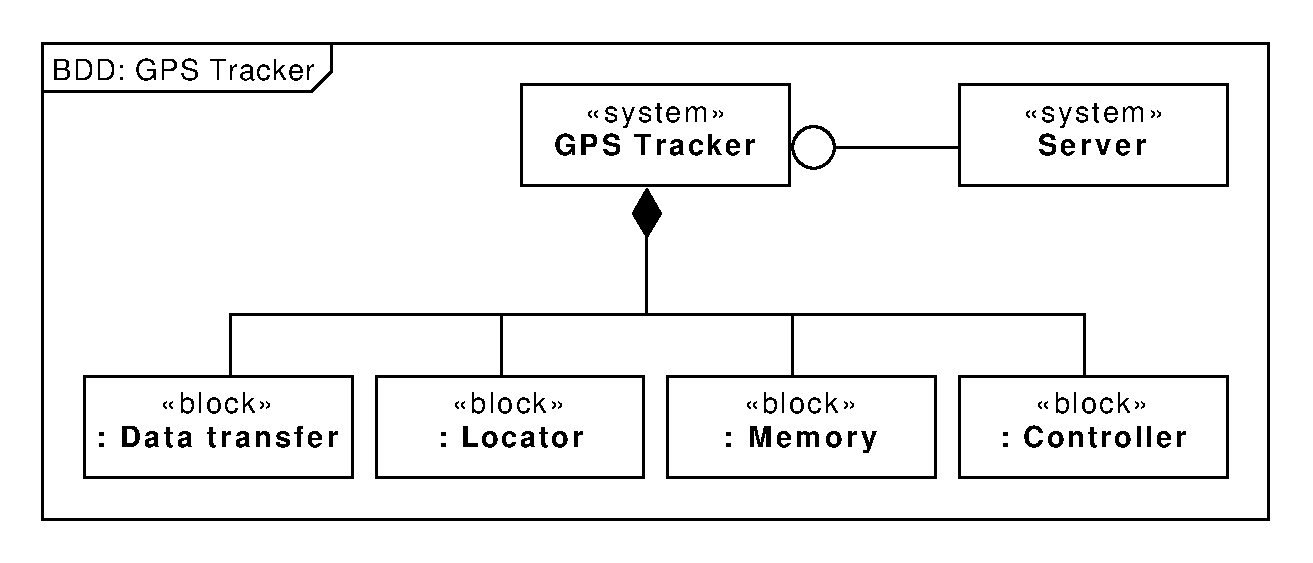
\includegraphics[width=0.7\linewidth]{gfx/Design/BDD_Unspecified.pdf}
	\caption{A high level BDD showing the parts of the \systemName, and the interface with a server.}
	\label{fig:BDD:unspecified}
\end{figure}

\section{Choice of components}
The physical entities necessary to solve the tasks of the blocks identified in \cref{fig:BDD:unspecified} are to be solved as follows:

\paragraph{Controller and Data transfer} can be performed by a single module. The \MKR which includes a SAM21D18A ARM µC and a u-blox SARA-U201-03B-00 High Speed Packet Access (HSPA) with 2G fallback module for internet access. They communicate using one of the two UARTs available on the SAM21D18A ARM µC.

\paragraph{Locator} has to be able to locate itself globally. This is solved using a GNSS module, u-blox NEO-7M-0-000, from Embedded Stock.
The module is able to use GPS (with SBAS and QZSS) and GLONASS, allowing for global positioning.
It also uses a maximum of \SI{67}{\milli\ampere} \cite[p.~17]{NEO7_Data} and is the low power version from the NEO-7 series.
The breakout-board
	
\section{\MKR}
Is the given Arduino board, with an ARM processor and a GSM module connected.

\subsection{µC - SAM21D18A}
The µC 

\subsection{GSM - SARA-U201-03B-00}
Connects with UART to the µC using serial port 5.

Can autodetect baudrates \num{1200}, \num{2400}, \num{4800}, \num{9600}, \num{19200}, \num{38400}, \num{57600}, \num{115200} and \num{230400}. Can also autodetect the frame configurations  7E1, 7O1, 8N1, 8E1 and 8O1.

Commands are send using the AT-commands listed below. The command is the string to send to the GSM module and the chapter is the chapter in \cite{ATcommands}, which corresponds to the command.

\begin{table}
	\begin{tabularx}{\textwidth}{l X X}
		\toprule
		Command & Description & Chapter \\
		\midrule
		+CPIN & Sim card pin commands & 9.1 \\
		+CCID & Sim card identification. Used for checking if the sim card is recognized. & 4.12 \\
		+CFUN & Module functionality. Includes power saving features. & 5.3 \\
		+CCLK & Get or set the real time clock. & 5.7 \\
		+CTZU & Automatic time zone setup. & 5.15 \\
		+CSQ & Check signal quality. & 7.2 \\
		+COPS & Operator selection and statys. & 7.4 \\
		+CGDCONT & APN and password setup. & 18.4 \\
		+CGATT & GPRS attach or detach. & 18.14 \\
		+CGACT & Activate or deactivate context. & 18.16 \\
		+CGREG & GPRS network registrations status & 18.27 \\
		+USOCO & Connect socket. & 25.9 \\
		+USOWR & Write to socket. & 25.10 \\
		+UPING & Ping command. & 30.1 \\
		\bottomrule
	\end{tabularx}
	\caption{Table of used AT commands.}
	\label{tab:ATcomm}
\end{table}
\fxnote{Check \url{http://m2msupport.net/m2msupport/data-call-at-commands-to-set-up-gprsedgeumtslte-data-call/} for expected behaviour.}

\section{GPS - NEO-7M-0-000}
Baud rates available: \num{4800}, \num{9600}, \num{19200}, \num{38400}, \num{57600} and \num{115200}. With frame 8N1.

\cite{MKRSchem}

\section{SD-card - Ciseco B026}

\FloatBarrier
